\documentclass[12pt]{article}
\usepackage{polski}
\usepackage[utf8]{inputenc}
\usepackage[margin=1in]{geometry}
\usepackage[english,polish]{babel}
\usepackage{graphicx}
\usepackage{indentfirst}
\usepackage{graphicx} 
\usepackage{float}
\usepackage{textcomp}
\usepackage{listings}
\usepackage{color}
\usepackage{hyperref}

\lstset{language=C++,
                keywordstyle=\color{blue},
                stringstyle=\color{red},
                commentstyle=\color{green},
                morecomment=[l][\color{magenta}]{\#},
                showspaces=false,
                showstringspaces=false
}

\begin{document}
\thispagestyle{empty}

\noindent
Mateusz Burniak, 218321 \\
Michał Bieroński, 218324 \\

\noindent
termin: pn, 16:10 \\
semestr: 2017/18 ZIMA

\vfill

\begin{center}
  \begin{Huge}
    Metody Techniki Systemów w Medycynie 2 \\
    \vspace{.5cm}
    projekt
  \end{Huge}
  
  \vspace{3cm}
  
  \begin{Large}
    Dokumentacja projektu: \\
    Analiza modelu jednokompartmentowego \\
    przy wlewie stałym
  \end{Large}
  
  \vspace{3cm}
  
  \begin{Large}
    Prowadzący: \\
Prof. dr hab. inż. Marek Kurzyński
  \end{Large}
  
  \vspace{3cm}
  
\end{center}

\vfill

OCENA:

\newpage

\section{Wstęp}

\subsection{Cel projektu}

Celem projektu jest poznanie modelu jednokompartmentowego oraz wykorzystanie go do analizy stężenia leku w organiźmie przy podawaniu go przez kroplówkę.

Dzięki naszej pracy możliwe będzie odpowiadanie na pytania:
\begin{itemize}
\item Jakie jest stężenie leku po $t$ minutach?
\item Po jakim czasie w organiźnie jest stężenie leku równe $c$ mg/ml?
\end{itemize}


\section{Badany problem}

\subsection{Model jednokompartmentowy}

Przy wlewie ze stałą prędkością poziom stężenia od czasu ma następującą postać:

\begin{equation}
\Large
c(t) = \frac{q}{k \cdot V} (1 - e^{-kt})
\end{equation}

Gdzie:

\begin{itemize}
\item $c$ - stężenie leku [mg/ml],
\item $t$ - czas [min],
\item $q$ - prędkość wlewu [ml/min],
\item $\frac {1}{k}$ - stała czasowa,
\item $V$ - objętość [ml].
\end{itemize}

\subsection{Dane empiryczne}

Zaaplikowano pacjentowi kroplówkę o stałej prędkości wlewu równej
$q = 1 \space ml/min$.

Następnie mierzono u pacjenta stężenia leku po 10, 30 i 120 minutach od rozpoczęcia procesu.

\begin{table}[H]
\caption{Dane zmierzone na pacjencie}
\center
\begin{tabular}{c|r|l}
& \large t [min] & \large c [mg/ml] \\
\hline
1 & 10 & 0.0019 \\
2 & 30 & 0.0052 \\
3 & 120 & 0.0140 \\
\end{tabular}
\end{table}

\subsection{Minimalizacja błędu}

Mając wzór na stężenie od czasu i dane empiryczne, możemy wyznaczyć nieznane parametry $k$ i $V$.
Należy rozwiązać zadanie regresji, by jak najlepiej dopasowa parametry do zmierzonych wartości.
Funkcja błędu, z której korzystamy, to błąd kwadratowy o wzorze:

\begin{equation}
Q(k, V) = \sum_{i=1}^{3} (c(t_i, k, V) - c_i) ^ 2
\end{equation}

Gdzie:

\begin{itemize}
\item $Q$ - wartość błędu,
\item $t_i$ - i-ta wartość czasu,
\item $c_i$ - i-ta wartość stężenia.
\end{itemize}

Zadanie sprowadza się do sprawdzenia dla jakich wartości parametrów $k$ i $V$ błąd przyjmuje wartość minimalną:

$$
\min_{k, V} Q(k, V) = ?
$$

W celu znalezienia dokładnych wartości parametrów najpierw należało zawęzić obszar poszukiwań.

Należało zacząć od wygenerowania dwóch szeregów liczb, osobno dla $k$ i $V$.
Dla $k$ były to liczby od 0 do 1 co 0.001, a $V$ od 0 do 10000 co 1.

Po zauważeniu, że błąd jest najmniejszy w okolicy $(k, V) = (0.010, 4988)$ i wynosi około $Q = 8.597 \cdot 10^{-11}$, zawęziliśmy obszar poszukiwań.

Drugim krokiem było szukanie w zakresach $k$ od 0.009 do 0.011 co $1 \cdot 10^{-6}$, a $V$ od 4500 do 5500 co 0.001.

Błąd wynosił około $Q = 8.221 \cdot 10^{-11}$ dla $(k, V) = (0.01002, 4986.522)$.
Wynik ten był satysfakcjonujący, dlatego zakończono poszukiwania.

\subsection{Wyniki}

\begin{figure}[H]                                 
\centering                                        
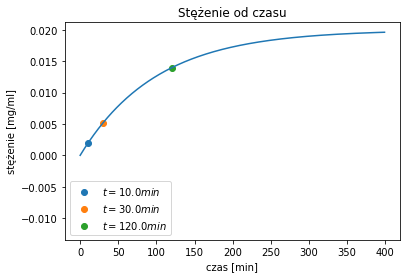
\includegraphics[scale=1.00]{c_t.png}   
\caption{Wykres stężenia od czasu}                      
\label{}                                          
\end{figure}                                      

\subsection{Zależność czasu od stężenia}

W celu umożliwienia odpowiedzi na wcześniej wymienione pytania należało wyznaczyć funkcję zależności czasu od podanego stężenia z funkcji stężenia od czasu.

\begin{equation}
t(c) = \frac{ln(1 - \frac{c \cdot k \cdot V}{q})}{-k}
\end{equation}

\subsection{Aplikacja interaktywna}

W aplikacji Jupyter Notebook stworzono interaktywny interfejs, gdzie można podając 
wartości czasu dowiedzieć się jakie będzie stężenie oraz podając stężenie można wyznaczyć po jakim czasie będzie osiągnięte.

\begin{figure}[H]                                 
\centering                                        
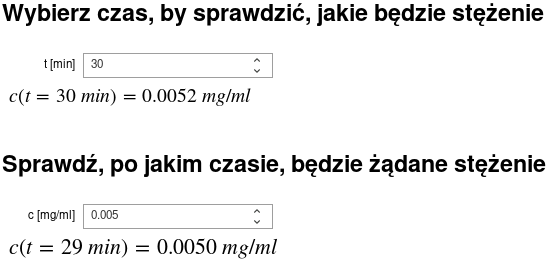
\includegraphics[scale=.65]{interfejs.png}   
\caption{Interaktywny interfejs}                      
\label{}                                          
\end{figure}  

\section{Wnioski}

Odpowiednie wykorzystanie wzoru na model jednokompartmentowy oraz danych empirycznych umożliwia znalezienie odpowiedzi na szereg pytań dotyczących stanu pacjenta.

Do wykonania projektu potrzebna była wiedza z kursu Metody Technik Systemów w Medycynie prowadzonego przez prof. Marka Kurzyńskiego oraz znajomość podstaw matematyki i programowania.

\section{Bibliografia}

\begin{itemize}
\item prezentacja z kursu MTSWM, Prof. dr hab. inż. Marek Kurzyński (2017)
\item \url{http://jupyter.org/widgets.html} (\today)

\end{itemize}

\end{document}
